\documentclass[11pt]{article}
\usepackage[a4paper,margin=1in]{geometry}
\usepackage{graphicx}
\usepackage{amsmath,amssymb}
\usepackage{booktabs}
\usepackage{longtable}
\usepackage{multirow}
\usepackage{hyperref}
\usepackage{enumitem}
\usepackage{xcolor}

\title{Modal Graph Analysis -- Final Report}
\author{Raphael des Boscs, Xufan Huang}
\date{April 2026}

\begin{document}
\maketitle
\tableofcontents
\newpage

\section{Abstract}
This report presents a multi-layer network analysis pipeline for AI repositories on GitHub.
Starting from topic-seeded repository retrieval (\texttt{computer-vision} and \texttt{nlp}), we construct a repository-level weighted graph, extract backbone structure, detect communities, and compute centrality metrics.
We then aggregate the repository graph to a company-level graph to evaluate whether ownership entities form distinct communities and whether small entities cluster together.
Methodologically, the project follows an iterative path: an initial topic-centric attempt on top100+top100 repositories, then single-signal experiments (fork-overlap only and README-similarity only), then a mixed-weight graph with community/centrality analysis, and finally company-level aggregation.
The report focuses on methodological design, explicit mathematical definitions, and reproducible implementation details.

\section{Research Questions}
We focus on the following questions:
\begin{enumerate}[leftmargin=1.5em]
    \item \textbf{RQ1}: Can a repository-level network built from fork, README, and dependency signals reveal interpretable AI communities at scale?
    \item \textbf{RQ2}: At company level, do ownership entities form distinct communities, and are these communities dominated by small entities?
    \item \textbf{RQ3}: Which repositories and companies play bridge roles across communities?
\end{enumerate}

\section{Data Acquisition and Cleaning}
\subsection{Sampling Strategy}
We use two query seeds on GitHub GraphQL:
\begin{itemize}[leftmargin=1.5em]
    \item \texttt{topic:computer-vision}
    \item \texttt{topic:nlp}
\end{itemize}
Our experiments were conducted in two stages:
\begin{itemize}[leftmargin=1.5em]
    \item \textbf{Stage A (initial repository-level run):} top \textbf{100+100} repositories (CV+NLP, about 200 raw repositories before deduplication), used to validate the repository-level graph pipeline and obtain the first interpretable repo communities.
    \item \textbf{Stage B (expanded company-level run):} because company communities from the 100+100 setting were too small/fragmented for stable interpretation, we expanded to top \textbf{500+500} repositories and reran the full pipeline for company-level analysis.
\end{itemize}
In Stage B, after cross-domain deduplication, the unique repository set contains \textbf{967 repositories}.

\subsection{Two-step GraphQL Retrieval}
To reduce request instability and payload size:
\begin{enumerate}[leftmargin=1.5em]
    \item \textbf{List stage}: retrieve compact repository metadata (\texttt{nameWithOwner}, stars, forks, language).
    \item \textbf{Detail stage}: per repository, retrieve topics, README text, dependency files, and forks.
\end{enumerate}

\subsection{GitHub GraphQL: Role in Our Study and Queries}
\paragraph{Brief introduction}
GitHub GraphQL is a typed query API where we request exactly the fields needed for each repository.
Compared with broad REST crawling, this reduces payload redundancy and enables nested retrieval (repository metadata, topics, README blobs, dependencies, forks) in a controlled schema.

\paragraph{Why it matters for this project}
It is the data backbone of our pipeline:
\begin{itemize}[leftmargin=1.5em]
    \item supports \textbf{topic-seeded sampling} for CV/NLP repositories;
    \item enables \textbf{two-step retrieval} (light list pass, then deep detail pass);
    \item provides the raw signals used in edge construction (\texttt{fork overlap}, \texttt{README similarity}, \texttt{dependency overlap}).
\end{itemize}

\paragraph{Search query string used in the list stage}
For each domain, we query:
\begin{verbatim}
topic:{domain} sort:stars-desc
\end{verbatim}
where \texttt{domain} is \texttt{computer-vision} or \texttt{nlp}.

\paragraph{GraphQL query used in the list stage (\texttt{LIST\_REPOS\_QUERY})}
\begin{verbatim}
query($searchQuery: String!, $cursor: String, $first: Int!) {
  search(query: $searchQuery, type: REPOSITORY, first: $first, after: $cursor) {
    pageInfo { hasNextPage endCursor }
    nodes {
      ... on Repository {
        nameWithOwner
        stargazerCount
        forkCount
        primaryLanguage { name }
      }
    }
  }
}
\end{verbatim}

\paragraph{GraphQL query used in the detail stage (\texttt{DETAIL\_QUERY})}
\begin{verbatim}
query(
  $owner: String!,
  $name: String!,
  $topicsFirst: Int!,
  $forksFirst: Int!
) {
  repository(owner: $owner, name: $name) {
    nameWithOwner
    stargazerCount
    forkCount
    isFork
    primaryLanguage { name }
    parent { nameWithOwner }
    repositoryTopics(first: $topicsFirst) {
      nodes { topic { name } }
    }
    readmeMd: object(expression: "HEAD:README.md") { ... on Blob { text } }
    readmeLower: object(expression: "HEAD:readme.md") { ... on Blob { text } }
    readmeRst: object(expression: "HEAD:README.rst") { ... on Blob { text } }
    readmeTxt: object(expression: "HEAD:README.txt") { ... on Blob { text } }
    readme: object(expression: "HEAD:README") { ... on Blob { text } }

    pkgJson: object(expression: "HEAD:package.json") { ... on Blob { text } }
    reqTxt: object(expression: "HEAD:requirements.txt") { ... on Blob { text } }
    pyprojectToml: object(expression: "HEAD:pyproject.toml") { ... on Blob { text } }
    goMod: object(expression: "HEAD:go.mod") { ... on Blob { text } }
    cargoToml: object(expression: "HEAD:Cargo.toml") { ... on Blob { text } }
    pomXml: object(expression: "HEAD:pom.xml") { ... on Blob { text } }
    gemfile: object(expression: "HEAD:Gemfile") { ... on Blob { text } }
    envYml: object(expression: "HEAD:environment.yml") { ... on Blob { text } }
    forks(first: $forksFirst) {
      totalCount
      nodes {
        nameWithOwner
        isArchived
        pushedAt
        stargazerCount
        owner { login }
      }
    }
  }
}
\end{verbatim}

\subsection{Raw Fields Collected}
Per repository, we collect:
\begin{itemize}[leftmargin=1.5em]
    \item Basic: \texttt{nameWithOwner}, \texttt{stargazerCount}, \texttt{forkCount}, \texttt{primaryLanguage}
    \item Content: README text (multiple path fallbacks)
    \item Dependencies: \texttt{requirements.txt}, \texttt{pyproject.toml}, \texttt{package.json}, \texttt{go.mod}, \texttt{Cargo.toml}, \texttt{pom.xml}, \texttt{Gemfile}, \texttt{environment.yml}
    \item Social signal: fork owners
    \item Domain context: source topic-domain assignment (CV / NLP / cross-domain)
\end{itemize}

\subsection{Cleaning Rules}
User/account filtering:
\begin{itemize}[leftmargin=1.5em]
    \item Remove any login containing \texttt{[bot]}
    \item Remove \texttt{web-flow}
\end{itemize}
Dependency names and company labels are normalized to reduce lexical duplication.

\section{Repository-level Graph Construction}
\subsection{Method Evolution (from Topics to Hybrid Similarity)}
We did \textbf{not} start directly from the final mixed-weight graph.
Instead, the repository-level design evolved in the following order:
\begin{enumerate}[leftmargin=1.5em]
    \item \textbf{Topic-centric trial on top100+top100 raw data}: we first attempted to organize repositories mainly by topic metadata.
    \item \textbf{Observation}: topic fields were noisy in practice (missing tags, inconsistent granularity, and heterogeneous naming), which made pure topic grouping unstable.
    \item \textbf{Signal shift}: we moved to structural/textual similarity, prioritizing fork-overlap and README semantic similarity.
    \item \textbf{Single-signal ablations}: we generated separate views with fork-overlap only and README-similarity only (figures to be inserted), then compared their strengths/limitations.
    \item \textbf{Final repository graph}: we adopted the hybrid weighting design and then applied backbone extraction + Louvain + centrality metrics.
\end{enumerate}
This evolution explains why topics are kept as attributes/context, but not used as the only relation signal.

\subsection{Node Definition}
Each node is a repository.
Topics are retained as node attributes (not topic nodes), avoiding excessive topic-projection density.

\subsection{Edge Weight Design}
For repositories $i,j$, edge weight is defined as:
\begin{equation}
w_{ij}=\alpha s^{\text{fork}}_{ij}+\beta s^{\text{readme}}_{ij}+\gamma s^{\text{dep}}_{ij}
\end{equation}
with default parameters:
\begin{equation}
(\alpha,\beta,\gamma)=(0.6,0.2,0.2)
\end{equation}

\paragraph{Fork-overlap signal}
\begin{equation}
s^{\text{fork}}_{ij}=\frac{|F_i\cap F_j|}{|F_i\cup F_j|}
\end{equation}
where $F_i$ is the set of fork-owner accounts of repository $i$.

\paragraph{README semantic signal}
README text is preprocessed (remove code blocks, markdown links/images, low-information terms), then converted into sparse TF-IDF vectors which is in dictionary form by representing every word with the TF-IDF score.
For term $t$ in document $d$:
\begin{equation}
\text{tfidf}(t,d)=\left(1+\log \text{tf}(t,d)\right)\left(\log\frac{1+N}{1+\text{df}(t)}+1\right)
\end{equation}
README similarity:
\begin{equation}
s^{\text{readme}}_{ij}=\frac{v_i\cdot v_j}{\|v_i\|\|v_j\|}
\end{equation}


\paragraph{Dependency-overlap signal}
\begin{equation}
s^{\text{dep}}_{ij}=\frac{|D_i\cap D_j|}{|D_i\cup D_j|}
\end{equation}
where $D_i$ is the parsed dependency set.

\section{Backbone Extraction and Denoising}
The raw similarity graph is filtered in stages:
\begin{enumerate}[leftmargin=1.5em]
    \item \textbf{Pre-threshold} (\texttt{pre-min-weight}) before edge insertion.
    \item \textbf{Backbone threshold} (\texttt{min-weight}) on existing edges.
    \item \textbf{Optional top-$k$ sparsification} per node.
    \item \textbf{Optional $k$-core pruning}.
\end{enumerate}

\subsection{Auto-relax Strategy}
To avoid graph collapse under strict thresholds, we evaluate multiple relaxed candidate configurations and select by a size--modularity utility.
This increases robustness for large and heterogeneous samples.

\section{Community Detection and Centrality}
\subsection{Louvain Community Detection}
Weighted Louvain is applied to the final backbone graph.
Node attribute \texttt{Community} stores cluster IDs.
Louvain greedily optimizes modularity:
\begin{equation}
Q=\frac{1}{2m}\sum_{i,j}\left(A_{ij}-\frac{k_i k_j}{2m}\right)\mathbf{1}(c_i=c_j)
\end{equation}
where $A_{ij}$ is weighted adjacency, $k_i$ is weighted degree, and $m$ is total edge weight.
Intuitively, Louvain prefers partitions with denser-than-random intra-community connectivity.

\subsection{Centrality Metrics}
We compute:
\begin{itemize}[leftmargin=1.5em]
    \item Weighted PageRank
    \item Weighted betweenness centrality (edge distance $=1/w$)
    \item Weighted eigenvector centrality
\end{itemize}
Interpretation used in this report:
\begin{itemize}[leftmargin=1.5em]
    \item \textbf{PageRank}: influence under recursive endorsement from important neighbors.
    \item \textbf{Betweenness centrality}: bridge score based on shortest paths crossing a node. For node $v$,
    \begin{equation}
    C_B(v)=\sum_{s\neq v\neq t}\frac{\sigma_{st}(v)}{\sigma_{st}}
    \end{equation}
    where $\sigma_{st}$ is the number of shortest paths from $s$ to $t$, and $\sigma_{st}(v)$ counts those passing through $v$.
    \item \textbf{Eigenvector centrality}: importance by being connected to other important nodes.
\end{itemize}
In practice, high-betweenness repositories/companies are interpreted as cross-community connectors.
These metrics are exported to GEXF for visualization and downstream analysis.

\section{Company-level Aggregation}
\subsection{Mapping Owner to Company}
Company entities are inferred from repository owner:
\begin{enumerate}[leftmargin=1.5em]
    \item If owner is an \textbf{Organization}, we use organization name/login as company identity.
    \item If owner is a \textbf{User}, we use the profile \texttt{company} field.
    \item Owners with no company information are removed for the final company graph.
\end{enumerate}

\subsection{Company Graph}
Company node features include:
\texttt{RepoCount}, \texttt{TotalStars}, \texttt{OwnerCount}, \texttt{SmallCompany} flag.

For company pair $(a,b)$, we aggregate repository edges and normalize:
\begin{equation}
W_{ab}=\frac{\sum_{(i,j)\in \mathcal{P}_{ab}} w_{ij}}{\sqrt{n_a n_b}}
\end{equation}
where $\mathcal{P}_{ab}$ are cross-company repository pairs and $n_a,n_b$ are repository counts per company.

Louvain is then applied again on the company graph, producing \texttt{CompanyCommunity}.
\paragraph{Weight semantics}
For each company-company edge, we keep both:
\begin{itemize}[leftmargin=1.5em]
    \item \texttt{raw\_weight}: direct sum of underlying repository-pair similarities;
    \item \texttt{weight}: normalized weight used in clustering and layout ($W_{ab}$ above).
\end{itemize}

\section{Results by Sampling Stage}
\subsection{Stage A: Initial Repository-level Analysis (100+100)}
Our repository-level exploration started from the 100+100 raw setting.
This stage was used to verify that the weighted repository graph and Louvain communities were meaningful, and to inspect bridge repositories before scaling.
However, when projected to company level, the resulting company communities were too small for robust interpretation.
Therefore, we kept Stage A for methodological validation and moved final company interpretation to Stage B.

\subsection{Stage B: Expanded Run for Company Analysis (500+500)}
\paragraph{Repository-level summary in Stage B}
\begin{table}[h]
\centering
\caption{Repository-level graph summary used for the expanded Stage B run (CV500 + NLP500)}
\begin{tabular}{lr}
\toprule
Metric & Value \\
\midrule
Unique repositories (after merge) & 967 \\
Backbone nodes & 847 \\
Backbone edges & 22,893 \\
Density & 0.063897 \\
Average path length (LCC) & 2.795839 \\
Communities & 19 \\
Modularity & 0.2576 \\
\bottomrule
\end{tabular}
\label{tab:repo-summary}
\end{table}

\paragraph{Company-level summary in Stage B (company-filtered run)}
\begin{table}[h]
\centering
\caption{Company-level graph summary (owners without company removed)}
\begin{tabular}{lr}
\toprule
Metric & Value \\
\midrule
Company nodes & 451 \\
Company edges & 9,010 \\
Company communities & 36 \\
Modularity & 0.2210 \\
\bottomrule
\end{tabular}
\label{tab:company-summary}
\end{table}

\subsection{Interpretation of the Five Largest Company Communities (Stage B)}
Current evidence indicates that the ownership graph has a heavy-tail structure:
many small entities and a few high-connectivity anchors.
The five largest company communities contain most nodes and should be prioritized for interpretation; tiny communities (size 1--3) are unstable and should not be over-interpreted.

\begin{table}[h]
\centering
\caption{Five largest company communities (updated run)}
\begin{tabular}{rrrr}
\toprule
Community ID & Company count & Small-company ratio & Median stars \\
\midrule
3 & 114 & 0.9649 & 2415.0 \\
2 & 81  & 0.9753 & 2040.0 \\
0 & 74  & 0.9595 & 1679.5 \\
4 & 70  & 0.9286 & 1687.5 \\
1 & 50  & 0.9000 & 2122.5 \\
\bottomrule
\end{tabular}
\label{tab:top-company-communities}
\end{table}
\subsection{Company Graph Interpretation (Final Figure)}
\begin{figure}[htbp]
\centering
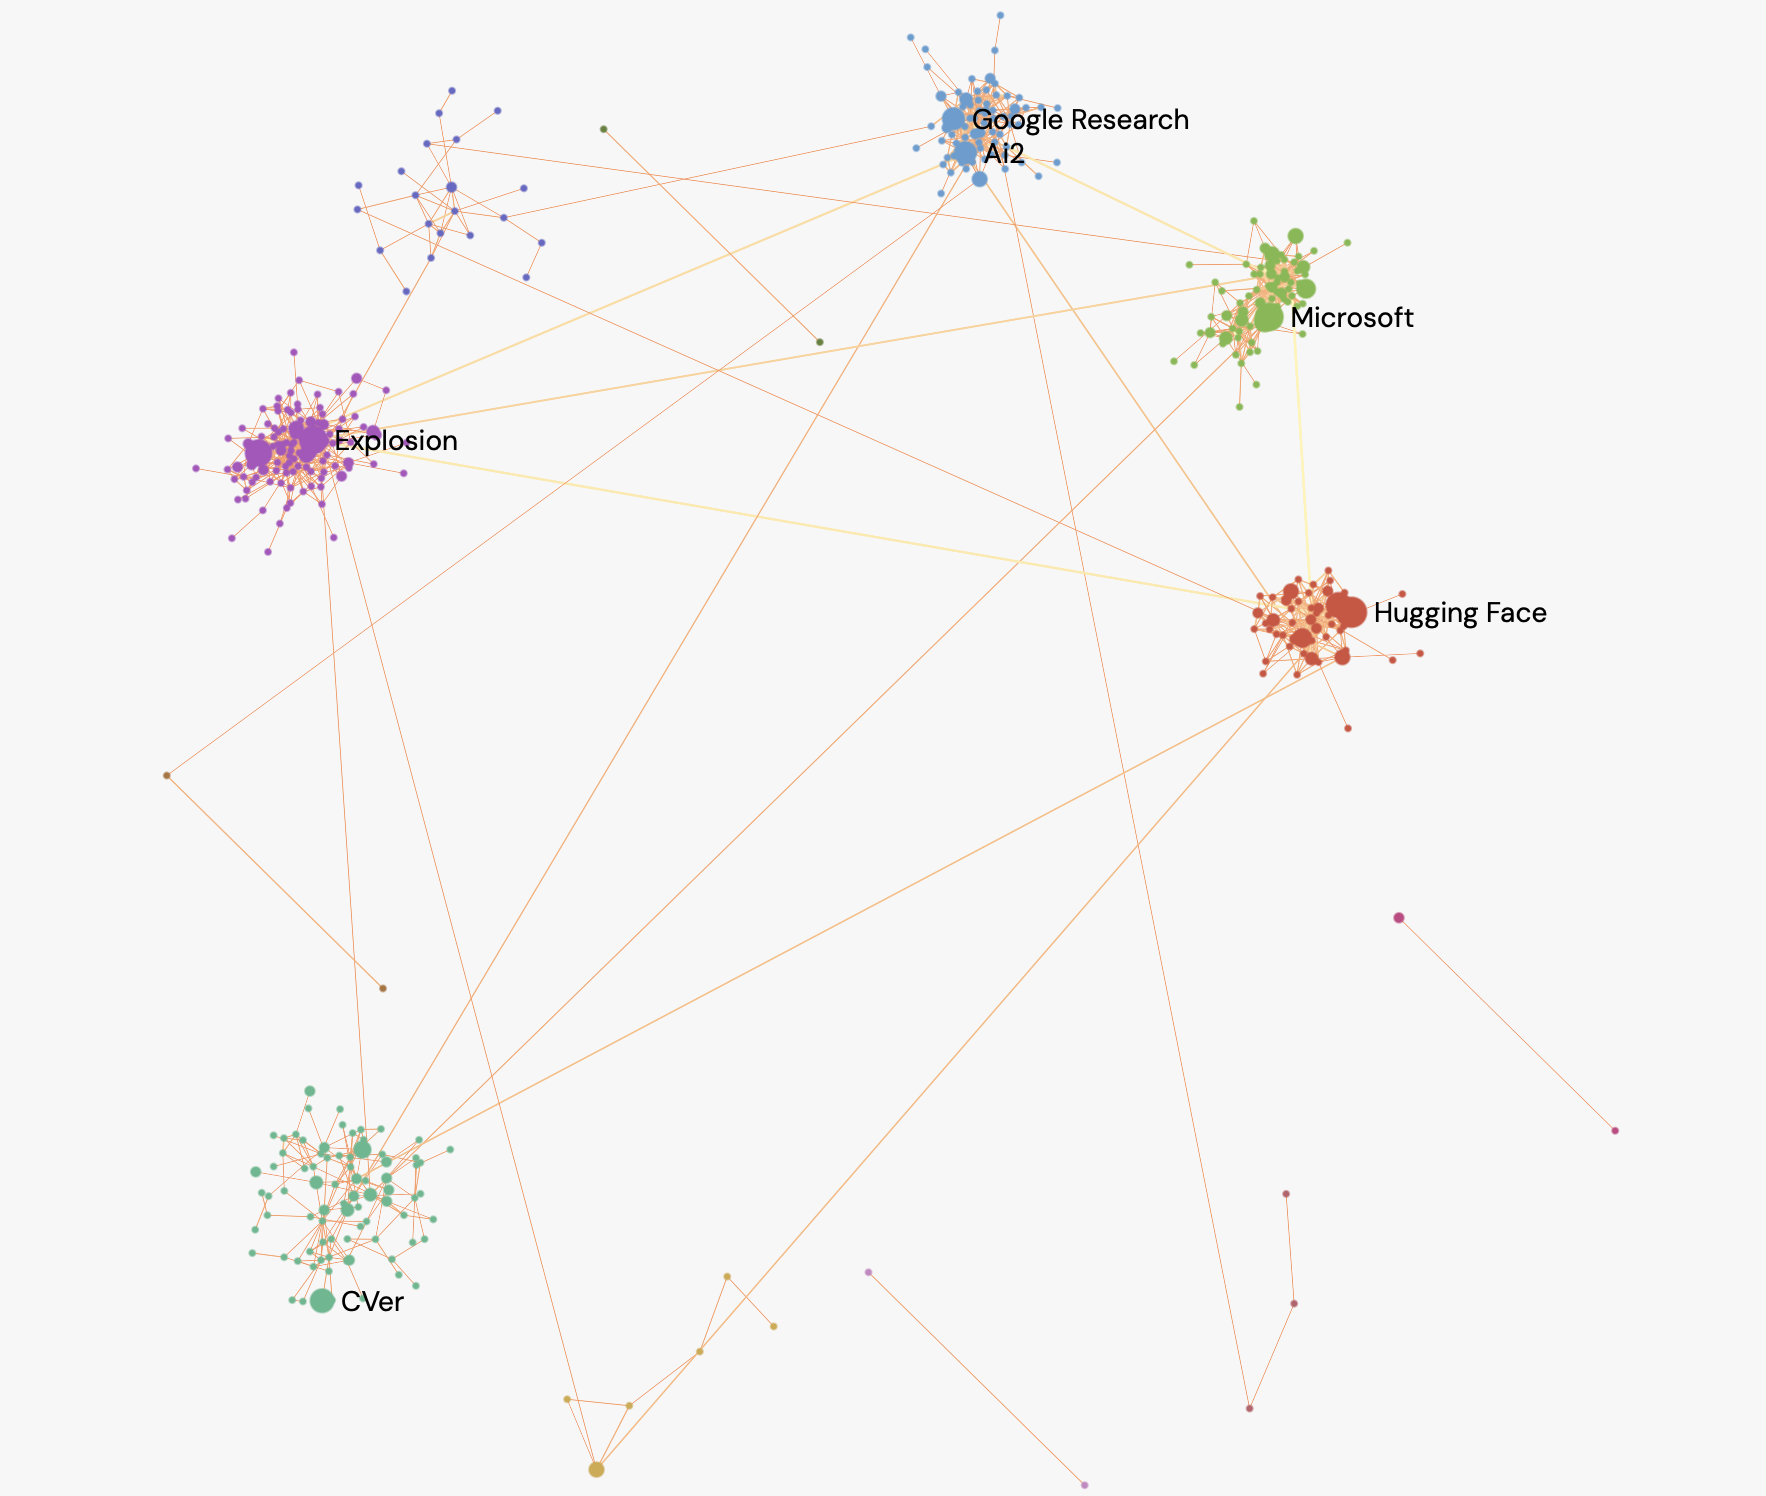
\includegraphics[width=0.94\linewidth]{figures/company_analysis.png}
\caption{Final company-level community graph used in our final analysis. Nodes are companies, node size reflects activity/importance, and node color indicates \texttt{CompanyCommunity}.}
\label{fig:company-analysis-final}
\end{figure}

\paragraph{How nodes are constructed}
Each node is a company entity derived from repository ownership after filtering:
\begin{itemize}[leftmargin=1.5em]
    \item organization owners are mapped directly to organization-level company IDs;
    \item user owners are mapped via profile \texttt{company};
    \item owners without company information are excluded.
\end{itemize}
Thus, the node set emphasizes identifiable organizations rather than anonymous personal accounts.

\paragraph{How edges are constructed}
For companies $a,b$, we aggregate all repository-level edges crossing the two companies:
\begin{equation}
\mathrm{raw\_weight}_{ab}=\sum_{(i,j)\in\mathcal{P}_{ab}} w_{ij}
\end{equation}
then normalize:
\begin{equation}
W_{ab}=\frac{\mathrm{raw\_weight}_{ab}}{\sqrt{n_a n_b}}
\end{equation}
where $n_a,n_b$ are repository counts of the two companies.
This prevents large entities from dominating simply due to scale.
In implementation, we keep an edge $(a,b)$ only when at least one cross-company repository pair contributes non-zero similarity; self-loops are removed.
Therefore, a company-company link means ``evidence of technical relatedness'' (fork overlap, README similarity, dependency overlap), not merely co-popularity.

\paragraph{Community meaning and examples}
The following interpretation is derived from \texttt{company\_network\_clustered\_compact.gexf} (451 nodes, 9010 edges), not only from visual proximity.
At the meso scale, communities \texttt{C0}, \texttt{C1}, \texttt{C3}, and \texttt{C4} form the structural core, while \texttt{C2} and most tiny communities behave as satellites.

\textbf{Core-vs-satellite evidence.}
The six strongest inter-community channels are
\texttt{C0-C4} (50.58), \texttt{C1-C4} (36.44), \texttt{C1-C3} (27.60),
\texttt{C0-C3} (27.59), \texttt{C3-C4} (26.04), and \texttt{C0-C1} (23.61).
Together they account for about 97\% of total cross-community edge weight.
In contrast, all links involving \texttt{C2} are much weaker
(\texttt{C2-C4}=1.36, \texttt{C0-C2}=1.21, \texttt{C2-C3}=0.95, \texttt{C1-C2}=0.94),
which quantitatively supports the ``peripheral CV enclave'' interpretation for \texttt{C2}.

\textbf{Community-level semantics with composition evidence.}
\begin{itemize}[leftmargin=1.5em]
    \item \textbf{C3 (114 nodes, dense applied NLP/CV tooling mix):} top repository owners include \textit{Explosion} (12 repos), \textit{Roboflow} (11), and \textit{Google} (4). High-betweenness nodes (\textit{Explosion}, \textit{DeepPavlov Team}) indicate this community is a major transit layer between productized tooling and other ecosystems.
    \item \textbf{C0 (74 nodes, research-platform transfer hub):} anchored by \textit{Ai2} (8), \textit{Google Research} (8), and \textit{PaddlePaddle} (4). Its strongest external coupling is toward \texttt{C4} and \texttt{C3}, suggesting a role as an upstream research source that diffuses methods into engineering communities.
    \item \textbf{C4 (70 nodes, industrial CV/infra engineering block):} anchored by \textit{Microsoft} (12), \textit{NVIDIA} (6), and \textit{Alibaba} (4). Strong coupling with \texttt{C0} and \texttt{C1} reflects continuous exchange between industrial deployment stacks and research/NLP model ecosystems.
    \item \textbf{C1 (50 nodes, model-hub and language-centric block):} centered on \textit{Hugging Face} (14), \textit{Tencent} (10), \textit{THUNLP} (6), and \textit{Bytedance Inc.} (4). It is internally cohesive and strongly connected to \texttt{C4} and \texttt{C3}, consistent with foundation-model tooling and multilingual NLP transfer.
    \item \textbf{C2 (81 nodes, sparse and specialized CV-oriented satellite):} although large in node count (\textit{CVer} and \textit{DAIR.AI} are prominent), it has low internal density and weak links to all core communities, indicating narrower technical overlap after normalization.
\end{itemize}

\textbf{Concrete bridge examples.}
High-weight cross-community edges include
\textit{@cohere-ai (C1)}--\textit{Explosion (C3)} (0.1448),
\textit{Autodistill (C0)}--\textit{Roboflow (C3)} (0.1274),
\textit{Ai2 (C0)}--\textit{DeepPavlov Team (C3)} (0.1120), and
\textit{Explosion (C3)}--\textit{@huggingface (C1)} (0.1126).
These bridges explain why the four-core-community block remains strongly integrated despite clear color-separated modules in Figure~\ref{fig:company-analysis-final}.

\section{Visualization Protocol}
\subsection{Why ``hairball'' happens}
Dense cross-community edges and high edge-count per node can collapse community separation under force-directed layouts.
To improve readability, we generated a clustered variant (\texttt{company\_network\_clustered.gexf}) by preserving strong intra-community links and only a small number of bridge edges.

\subsection{Recommended Gephi Layout Template}
\begin{itemize}[leftmargin=1.5em]
    \item Layout: ForceAtlas2
    \item LinLog mode: ON
    \item Prevent overlap: ON
    \item Gravity: 0.05
    \item Scaling: 180
    \item Edge weight influence: 3.5
    \item Dissuade hubs: ON
    \item Then run Noverlap
\end{itemize}
Color nodes by \texttt{CompanyCommunity}, size nodes by \texttt{RepoCount} or \texttt{PageRank}.

\section{Figures and Tables To Insert}
\textbf{You can add the following additional assets to extend the experimental section:}
\begin{enumerate}[leftmargin=1.5em]
    \item \textbf{Figure F1}: Repository graph from fork-overlap only (single-signal ablation).
    \item \textbf{Figure F2}: Repository graph from README-similarity only (single-signal ablation).
    \item \textbf{Figure F3}: Final repository backbone network (hybrid weight; colored by \texttt{Community}, sized by PageRank).
    \item \textbf{Figure F4}: Company network raw (\texttt{company\_network.gexf}) for density comparison.
    \item \textbf{Figure F5}: Company network clustered (\texttt{company\_network\_clustered.gexf}) for interpretability.
    \item \textbf{Figure F6}: Community meta-graph (if used), showing inter-community connectivity.
    \item \textbf{Table T1}: Parameter sensitivity (weight mix, threshold, top-$k$, $k$-core, resolution) vs modularity.
    \item \textbf{Table T2}: Top bridge repositories and top bridge companies by weighted betweenness.
    \item \textbf{Table T3}: Domain composition per community (CV/NLP/Cross).
\end{enumerate}

\begin{figure}[h]
\centering
\fbox{\parbox[c][2.2in][c]{0.9\linewidth}{\centering Placeholder for additional repository-level graph (optional)}}
\caption{Optional additional repository-level graph view.}
\label{fig:repo-graph}
\end{figure}

\section{Threats to Validity}
\begin{itemize}[leftmargin=1.5em]
    \item \textbf{Company identity noise}: profile \texttt{company} fields are user-provided and can be missing, inconsistent, or stylistically heterogeneous.
    \item \textbf{Sampling bias}: top-star sampling over-represents popular repositories.
    \item \textbf{Metadata incompleteness}: README and dependency files are not uniformly available.
    \item \textbf{Method sensitivity}: community assignments depend on backbone and resolution parameters.
    \item \textbf{Temporal bias}: single snapshot may hide dynamics of ecosystem evolution.
\end{itemize}

\section{Reproducibility}
\subsection{Environment}
Conda environment: \texttt{cours}. Required libraries include:
\texttt{requests}, \texttt{networkx}, \texttt{pandas}, \texttt{python-louvain}.

\subsection{Main Commands}
\paragraph{Stage A (initial repository-level run, 100+100)}
\begin{verbatim}
python scripts/build_repository_backbone.py \
  --raw-output data/raw/repo_raw_data_fork.json \
  --gexf-output outputs/graphs/repo/repository_backbone_fork.gexf \
  --per-domain-limit 100 \
  --weight-fork 0.6 --weight-readme 0.2 --weight-dep 0.2
\end{verbatim}

\paragraph{Stage B (expanded run for company analysis, 500+500)}
\begin{verbatim}
python scripts/build_repository_backbone.py \
  --raw-output data/raw/repo_raw_data_fork.json \
  --gexf-output outputs/graphs/repo/repository_backbone_fork.gexf \
  --per-domain-limit 500 \
  --weight-fork 0.6 --weight-readme 0.2 --weight-dep 0.2
\end{verbatim}

\paragraph{Company aggregation (used in Stage B)}
\begin{verbatim}
python scripts/analyze_company_communities.py \
  --repo-raw data/raw/repo_raw_data_fork.json \
  --repo-graph outputs/graphs/repo/repository_backbone_fork.gexf \
  --company-graph outputs/graphs/company/company_network.gexf \
  --company-nodes-csv outputs/tables/company_nodes.csv \
  --company-communities-csv outputs/tables/company_communities.csv \
  --owner-company-map-csv outputs/tables/owner_company_map.csv \
  --fetch-owner-company \
  --drop-owners-without-company
\end{verbatim}

\section{Conclusion}
We implemented and validated an end-to-end, scalable graph-analysis pipeline from repository retrieval to company-level community aggregation.
The current results support a structured ecosystem with multiple large ownership communities and high prevalence of small entities.
Next steps should focus on (i) stronger owner-to-company normalization, (ii) parameter robustness experiments, and (iii) temporal analysis for community evolution.

\end{document}
